\section{(2.9)}
% The National Research Council has decided to pursue research in the area of spray-dried
% agglomeration of nano-sized powder particles to produce micron-sized powder particles. Safety and
% health regulations permit only a limited amount of these particles to escape into the ambient air of
% the space. To that end, the Council has contracted the services of Alliance Engineering Corp. to
% design a high-velocity duct system using a Farr® Gold Series 10 dust collector. The dust collector
% will draw 4000 cfm of air to eliminate powder particles from the space. The air will be drawn through
% a hood and the dust collector, as shown below, with dimensions. The dust collector and hood have a
% total pressure loss of 2.7 in. w.g. The Council will provide a lab environment with a maximum duct
% velocity of 2500 to 6000 fpm.
% a) Design and size round ductwork between the hood and the dust collector (the duct layout,
% accessories, and fittings).
% b) Select an appropriate Greenheck 15 BISW fan (identify nominal fan speed and motor power).

\textit{The National Research Council has decided to pursue research in the area of spray-dried agglomeration of nano-sized powder particles to produce micron-sized powder particles. Safety and health regulations permit only a limited amount of these particles to escape into the ambient air of the space. To that end, the Council has contracted the services of Alliance Engineering Corp. to design a high-velocity duct system using a Farr® Gold Series 10 dust collector. The dust collector will draw 4000 cfm of air to eliminate powder particles from the space. The air will be drawn through a hood and the dust collector, as shown below, with dimensions. The dust collector and hood have a total pressure loss of 2.7 in. w.g. The Council will provide a lab environment with a maximum duct velocity of 2500 to 6000 fpm.}

\begin{figure}[H]
\centering
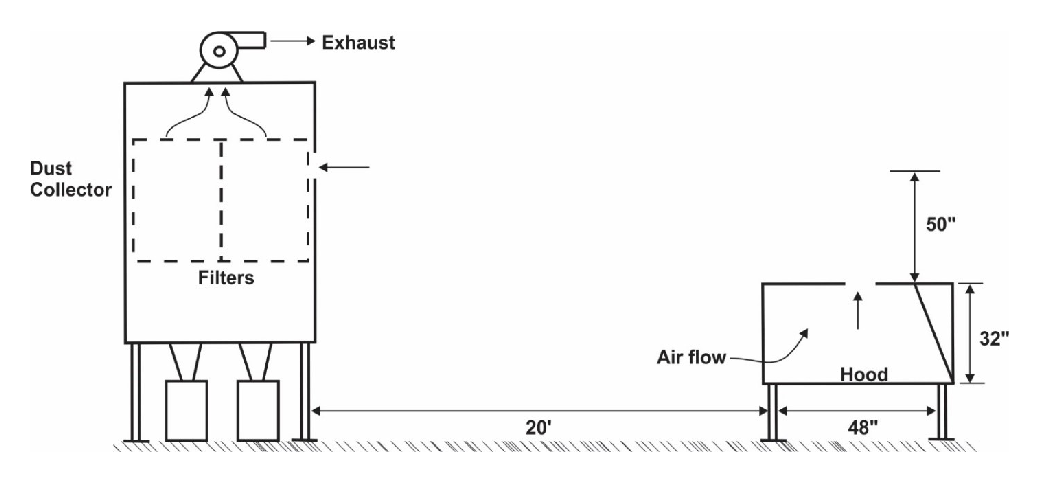
\includegraphics[width=0.9\textwidth]{Questions/Figures/Q2 Problem.png}
\end{figure}

\paragraph{a)} \textit{Design and size round ductwork between the hood and the dust collector (the duct layout, accessories, and fittings).}
\subsection{Assumptions}
\begin{enumerate}
    \item Bellmouth used at both the hood and the dust collector.
    \item Round ductwork system
    \item The elbow is pleated 90$^\circ$.
    \item Galvanized steel duct material is used (common in air ducts).
    \item The airflow is 4000 cfm.
    \item The pressure loss for the hood and dust collector is 2.7 in. w.g.
\end{enumerate}
\subsection{Sketches}
\begin{figure}[H]
\centering
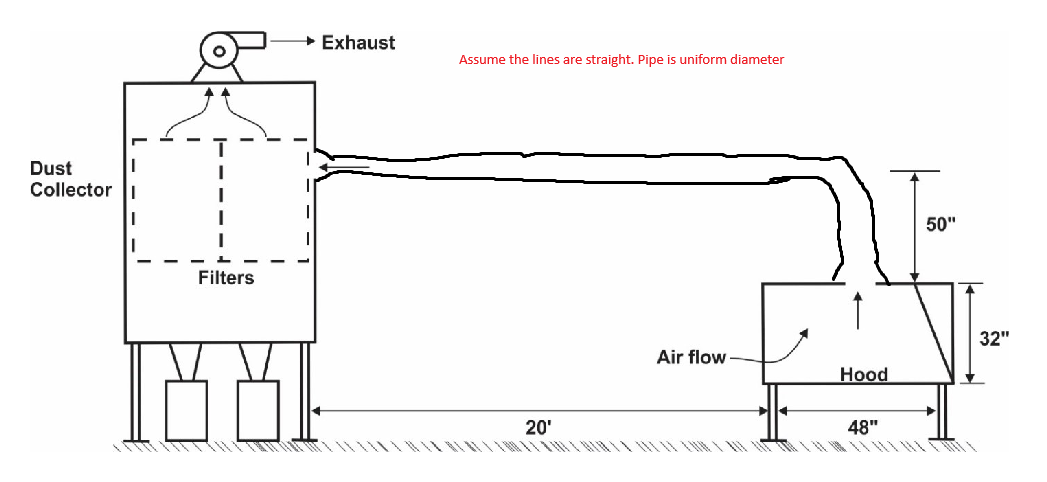
\includegraphics[width=0.9\textwidth]{Questions/Figures/Q2 Sketch.png}
\end{figure}
\subsection{Analysis}
\subsubsection{Determine Air Velocity}
From Table 2.3
\begin{figure}[H]
\centering
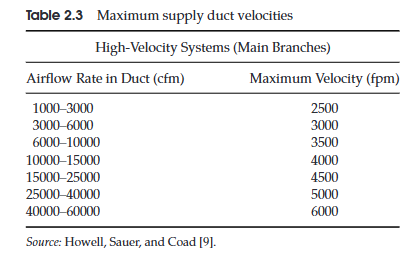
\includegraphics[width=0.9\textwidth]{Questions/Figures/Q2 Table 2.3.png}
\end{figure}
It is clear the maximm velocity is 3000 fpm. This is within the range of 2500 to 6000 fpm.

\subsubsection{Determine Duct Diameter}
Using A.1:
\begin{figure}[H]
\centering
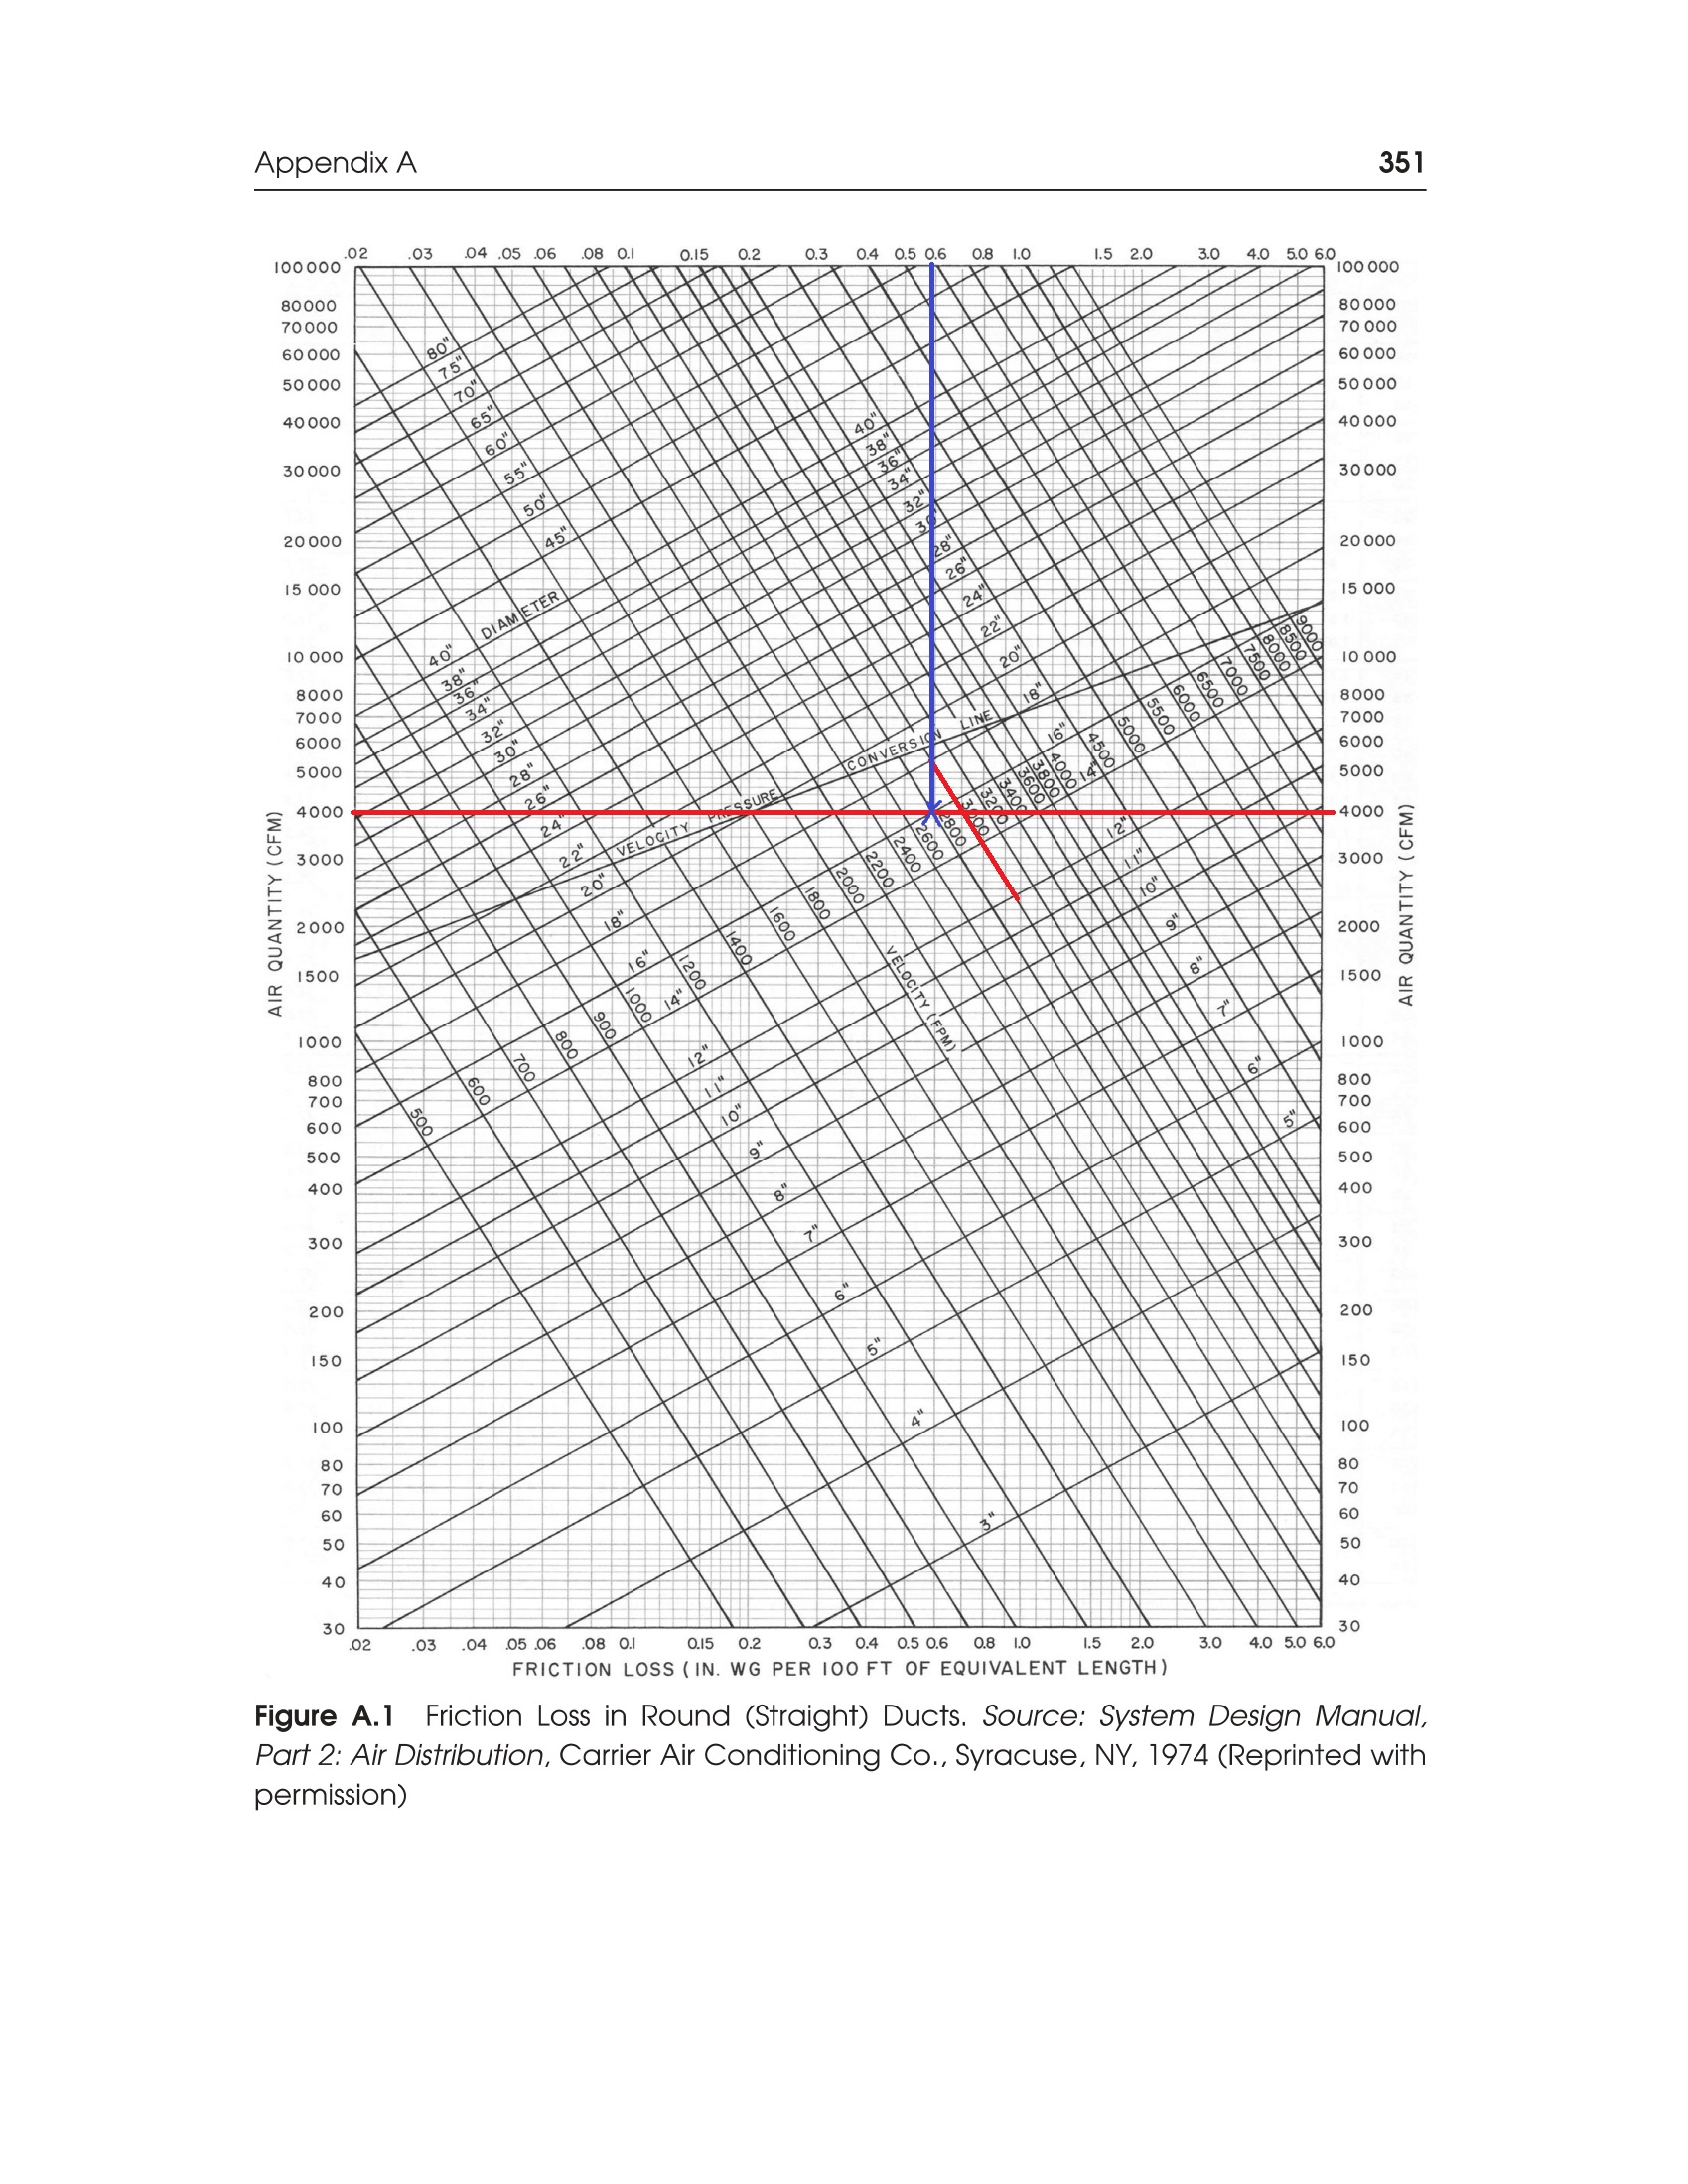
\includegraphics[width=0.9\textwidth]{Questions/Figures/Q2 A.1.jpg}
\end{figure}
From the chart, 16'', 2800 fpm, 0.6 in. wg. per 100ft. is the closest to the design conditions. 

\subsubsection{Determine Equivalent Length}
The length of the straight portions are
\begin{align*}
    L_{\text{straight}} &= 20' + \frac{48''}{2} + 50'' = 20' + 2' + 4.17' = 26.17'
\end{align*}
The equivalent length of the elbow is
\begin{align*}
    L_{\text{elbow}} &= 16'' \cdot 15 = 240'' = 20'
\end{align*}
The equivalent length of the bellmouths are
\begin{align*}
    L_{\text{bellmouth, hood}} = L_{\text{bellmouth, col}}  &= 16'' \cdot 12
   &= 192'' = 16'
\end{align*}
The total equivalent length is
\begin{align*}
    L_{\text{total}} &= L_{\text{straight}} + L_{\text{elbow}} + L_{\text{bellmouth, hood}} + L_{\text{bellmouth, col}} \\
    &= 26.17' + 20' + 16' + 16' 
    &= 78.17'
\end{align*}

\subsubsection{Determine Pressure Loss}
The presure drop from the duct is 
\begin{align*}
    \Delta P_{\text{duct}} &= \frac{0.6}{100} \cdot 78.17' = 0.47 \text{ in. w.g.}
\end{align*}
The total pressure drop is
\begin{align*}
    \Delta P_{\text{total}} &= \Delta P_{\text{duct}} + \Delta P_{\text{hood+col}} \\
    &= 0.47 + 2.7 \\
    &= 3.17 \text{ in. w.g.}
\end{align*}

\subsection{Conclusion}
The ductwork should be 16'' in diameter. The fan should be able to handle a pressure drop of 3.17 in. w.g. and a flow rate of 4000 cfm.

\paragraph{b)} \textit{Select an appropriate Greenheck 15 BISW fan (identify nominal fan speed and motor power).}
\setcounter{subsection}{0}
\subsection{Fan Selection}
The fan should move at least 4000 cfm and support a pressure drop of 3.17 in. w.g. Based on the performance curves, a nominal fan of 3100 rpm and 5 hp motor is the smallest specification that meets the requirements.
\begin{figure}
\centering
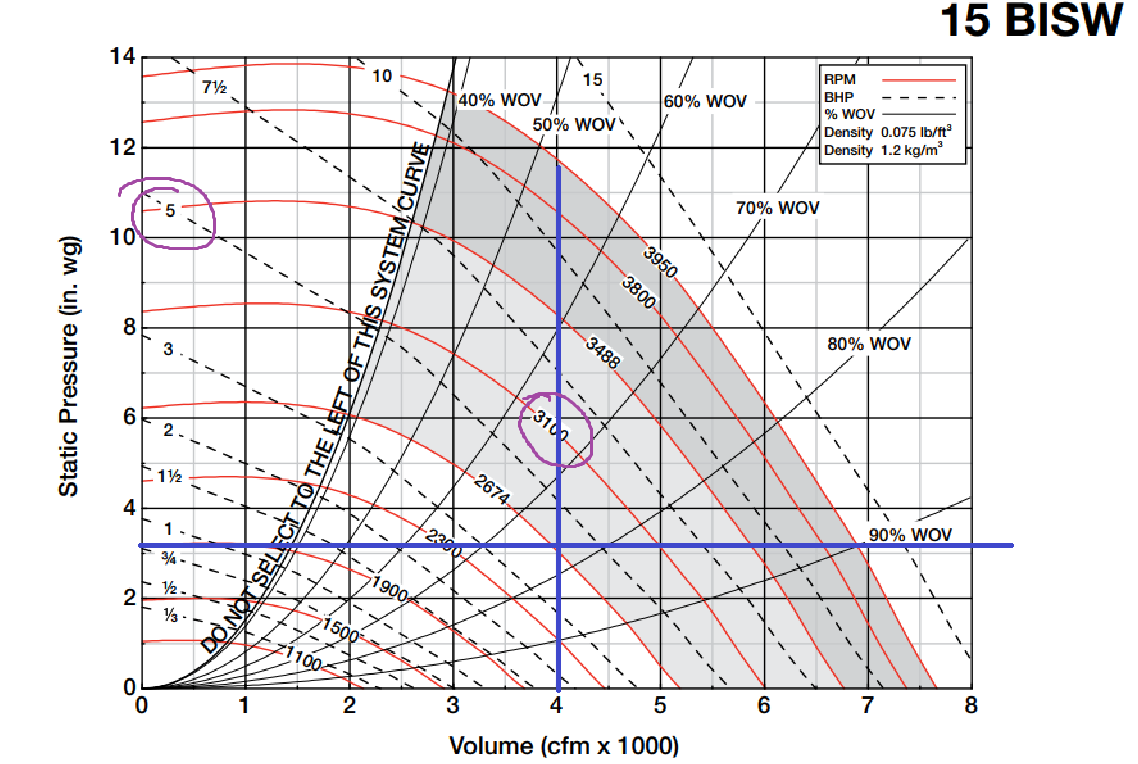
\includegraphics[width=0.9\textwidth]{Questions/Figures/Q2 Fan Chart.png}
\end{figure}
\subsection{Drawings}
\begin{figure}[H]
\centering
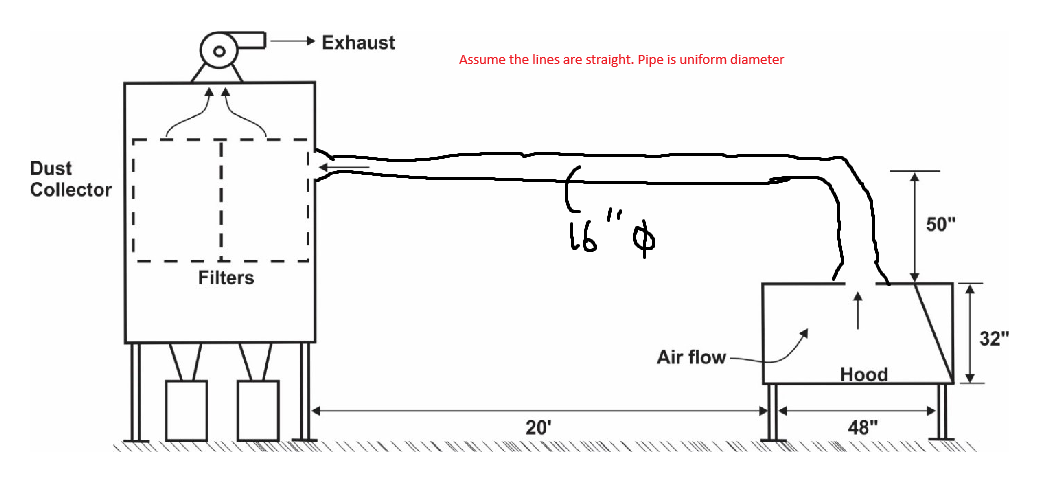
\includegraphics[width=0.9\textwidth]{Questions/Figures/Q2 Drawing.png}
\end{figure}
\subsection{Conclusion}
A round duct of 16'' has been selected for this project based on a required airflow of 4000 cfm and a maximum air velocity of 3000 fpm. 

A pleated 90$^\circ$ elbow is used to connect the hood to the dust collector. A bellmouth is used at both the hood and the dust collector. A smooth 90$^\circ$ elbow would prevent dust from accumulating in the ductwork and should be considered in further work.
